\documentclass[12pt]{article}
\usepackage[brazilian]{babel}
\usepackage[bottom=2.0cm,top=2.0cm,left=2.0cm,right=2.0cm]{geometry}
%\usepackage{fontspec}
\usepackage{indentfirst}
\usepackage{hyperref}
\usepackage{listings}
\usepackage[acronym, toc]{glossaries}
\usepackage{graphicx}

\AddToHook{cmd/section/before}{\clearpage}
\setkeys{Gin}{width=\linewidth}

%\setmainfont{Times New Roman}
\linespread{1.25}
\parindent=1.25cm

\renewcommand{\lstlistingname}{Código}
\renewcommand{\lstlistlistingname}{Lista de códigos}
\lstset{
  language=Python,
  frame=single,
  framerule=0pt,
  framextopmargin=3ex,
  framexbottommargin=3ex,
  framexleftmargin=1em,
  xleftmargin={\dimexpr 1em+3pt},
  breaklines=true,
}

\hypersetup{colorlinks,citecolor=black,filecolor=black,linkcolor=black,urlcolor=black}

\title{Modelo do LENS com RNA}
\author{Jaedson Barbosa Serafim}
\date{Outubro 2022}

\makeatletter
\renewcommand*{\fps@figure}{ht}
\renewcommand*{\fps@table}{ht}
\makeatother

\makeglossaries
\newacronym{rna}{RNA}{Rede Neural Artificial}
\newacronym{mse}{MSE}{Mean Squared Error, ou Erro Quadrático Médio}
\newacronym{mape}{MAPE}{Mean Absolute Percentage Error, ou Erro Percentual Absoluto Médio}

\begin{document}

\maketitle

\begin{abstract}

O objetivo deste trabalho é o desenvolvimento de uma RNA que preveja as vazões de dois pontos de medição do LENS usando como base a frequência do inversor da bomba e os valores atuais de vazão.
Neste relatório serão descritos todos os elementos usados para geração das \acrshort{rna}s responsáveis pelas previsões mostradas nas figuras aqui apresentadas.

Todo o código fonte deste projeto está escrito em Python e disponível no repositório do GitHub 
\href{https://github.com/jaedson-barbosa/modelagem-lens-rna}{jaedson-barbosa/modelagem-lens-rna}.

Vale ressaltar que não é objetivo deste relatório explicar sobre o funcionamento das \acrlong{rna} ou de como é feito seu treinamento/testes, aqui está escrito apenas um pequeno resumo sobre o que foi feito e subentende-se que o leitor tem total domínio sobre a linguagem Python e as bibliotecas aqui utilizadas. 

\end{abstract}

\tableofcontents

\section{Dados coletados}

\begin{table}
\caption{Arquivos fornecidos para testes}
\centering
\begin{tabular}{|l|l|} 
\hline
Nome & Descrição \\ 
\hline
initial & Medições com ângulo fixo em 0 e frequência variável \\ 
\hline
complete & Medições com frequência e ângulo variáveis \\
\hline
\end{tabular}
\label{tab:arquivos_testes}
\end{table}

\begin{table}
\caption{Arquivos fornecidos para treinamento}
\centering
\begin{tabular}{|l|l|} 
\hline
Nome & Descrição \\ 
\hline
0deg & Medições com ângulo fixo em 0 e frequência variável \\ 
\hline
30hz & Medições com frequência fixa em 30 Hz e ângulo variável \\ 
\hline
35hz & Medições com frequência fixa em 35 Hz e ângulo variável \\ 
\hline
40hz & Medições com frequência fixa em 40 Hz e ângulo variável \\ 
\hline
45hz & Medições com frequência fixa em 45 Hz e ângulo variável \\ 
\hline
50hz & Medições com frequência fixa em 50 Hz e ângulo variável \\
\hline
\end{tabular}
\label{tab:arquivos_treinamento}
\end{table}

As tabelas \ref{tab:arquivos_testes} e \ref{tab:arquivos_treinamento} contêm o nome e uma breve descrição de cada um dos arquivos fornecidos para a execução deste trabalho. Vale salientar que os nomes aqui apresentados não são exatamente iguais aos originais enviados pelo professor para fins de encurtamento de código.

A principal diferença entre os arquivos de treinamento e os arquivos de teste é que os valores de frequência e ângulo usados são diferentes, pois enquanto nos arquivos de treinamento foi usado um passo fixo de 5 unidades entre cada atualização da planta, em frequência do inversor ou ângulo da válvula, nos arquivos de teste o passo não teve valor fixo.
A principal razão desta diferença é que assim a \acrshort{rna} pôde ter sua capacidade de previsão realmente testada, pois é necessária um bom grau de generalização para que os valores que não foram treinados sejam corretamente previstos.

\section{Leitura e preparação de dados}

\lstinputlisting[label=code:importacao, caption={Importação das bibliotecas Pandas e NumPy}, firstline=1, lastline=2]{readdata.py}

Para a leitura e processamento de dados foram escolhidas as bibliotecas Pandas e NumPy, importadas como mostrado no código \ref{code:importacao}, por serem as opções mais populares para tal tarefa.

\lstinputlisting[label=code:renomeacoes, caption={Renomeações de colunas}, firstline=4, lastline=27]{readdata.py}

Para facilitar a leitura do código, os nomes inválidos de colunas dos arquivos XLSX fornecidos foram renomeados segundo o objeto definido no trecho de código \ref{code:renomeacoes}.

\lstinputlisting[label=code:leitura, caption={Funções de leitura de arquivos}, firstline=30, lastline=49]{readdata.py}

Para a leitura dos dados foram definidas as funções \textit{read\_training\_data} e \textit{read\_test\_data}, que servem apenas para apontar o caminho correto de arquivo para a função \textit{read\_excel} de acordo com o tipo de dado desejado, se é de treinamento ou de teste, como mostrado em \ref{code:leitura}.

Todas as funções possuem um parâmetro opcional \textit{add\_angle}, responsável por definir se o conjunto de dados em questão deve conter a informação de ângulo da válvula. A utilidade deste parâmetro será melhor entendida em seções posteriores, quando essa flexibilidade será requisitada.

\lstinputlisting[label=code:delay, caption={Função de adição de vazões atrasadas}, firstline=52, lastline=57]{readdata.py}

Todos os modelos treinados têm como parâmetro a vazão atual para poderem prever a próxima vazão, por isso a necessidade da função \textit{concat\_delayed\_flows} mostrada em \ref{code:delay}, responsável pela adição dessas vazões atrasadas.

\lstinputlisting[label=code:conversao, caption={Função de conversão e filtragem de dados}, firstline=60, lastline=66]{readdata.py}

Por fim, o código \ref{code:conversao} contêm a função responsável pela conversão do \textit{DataFrame} do Pandas para um vetor do NumPy, dividir a matriz entre entrada e saída e remover todos os erros dos sensores, ou seja, todas as vazões iguais ou menores que zero.
Novamente aqui existe o parâmetro \textit{with\_angle}, que deve ser igual àquele usado nas funções anteriores.

\section{Treinamento e checagem de modelo}

\lstinputlisting[label=code:importacao2, caption={Importação das bibliotecas TensorFlow e NumPy}, firstline=1, lastline=2]{model.py}

Novamente nesta seção é necessário usar funções da biblioteca Numpy, porém , como mostrado em \ref{code:importacao2}, aqui também é importada a biblioteca TensorFlow, responsável por todas as tarefas relacionadas ao treinamento e uso da \acrshort{rna}.

\lstinputlisting[label=code:treinamento, caption={Função de treinamento}, firstline=5, lastline=22]{model.py}

O código \ref{code:treinamento} mostra a função de treinamento, que tem como entradas: \textit{x} (entradas da \acrshort{rna}), \textit{y} (saídas esperadas da \acrshort{rna}), \textit{size} (número de variáveis de entrada), \textit{dense\_units} (vetor com quantidade de neurônios em cada camada oculta), \textit{epochs} (número de épocas usadas no treinamento) e \textit{name} (nome do modelo, será usado no arquivo gerado).

% MELHORAR

\lstinputlisting[label=code:load, caption={Função de carregamento de \acrshort{rna} já treinada}, firstline=24, lastline=26]{model.py}

Gerar uma boa \acrshort{rna} não é uma tarefa fácil, por isso é necessário ter a capacidade de recuperar todas as redes geradas, tarefa essa desempenhada pela função mostrada no código \ref{code:load}.

\lstinputlisting[label=code:check, caption={Função de checagem de \acrshort{rna}}, firstline=28, lastline=33]{model.py}

São usados como parâmetros de validação da rede neural o \acrfull{mse} e o \acrfull{mape}, cujo cálculo é feito pela função exibida em \ref{code:check}. Além dos dois parâmetros citados anteriormente, também é retornado por esta função os valores previstos para que possam ser exibidos como descrito na seção \ref{sec:exibicao}.

\section{Exibição de resultados}
\label{sec:exibicao}

\lstinputlisting[label=code:plotagem, caption={Importação da biblioteca Matplotlib e definição de funções de plotagem de dados}]{plotdata.py}

Para ter uma melhor ideia de como a \acrshort{rna} está se comportando é interessante uma análise visual dos dados e isso é feito por meio das duas funções especificadas no código \ref{code:plotagem}, que são responsável por gerar os gráficos relevantes para este relatório e para isso usam a biblioteca Matplotlib, escolha mais popular para esta finalidade.

\section {Criação do primeiro modelo}
\label{sec:modelo1}

\lstinputlisting[label=code:modelo1, caption={Geração do modelo 1}]{initial.py}

Para o treinamento deste primeiro modelo foi usado o arquivo \textit{0deg}, gerado da coleta de dados onde o inversor trabalhou com frequência fixa em 30 Hz e a variação de vazões foi provocada unicamente por causa da variação do ângulo de uma das válvulas da planta.

Como pode ser visto no código \ref{code:modelo1}, a \acrshort{rna} escolhida possui apenas uma camada oculta com 3 neurônios e foram usadas apenas 100 épocas para chegar a um \acrshort{mse} igual a 0,84 e um \acrshort{mape} de 11\%. Aumentar a quantidade de neurônios, camadas ocultas e/ou épocas não melhorou o resultado, muitas vezes os resultados encontrados foram inclusive piores.

\begin{figure}
    \centering
    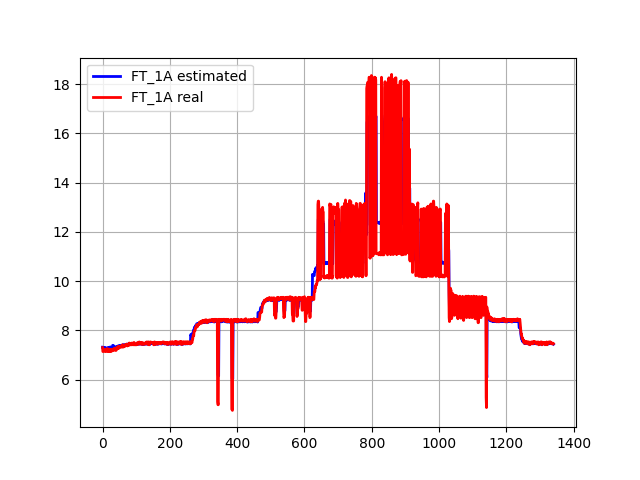
\includegraphics{results/initial-training-1A.png}
    \caption{Previsão da vazão 1A usando os dados de treinamento}
    \label{fig:initial-training-1A}
\end{figure}

\begin{figure}
    \centering
    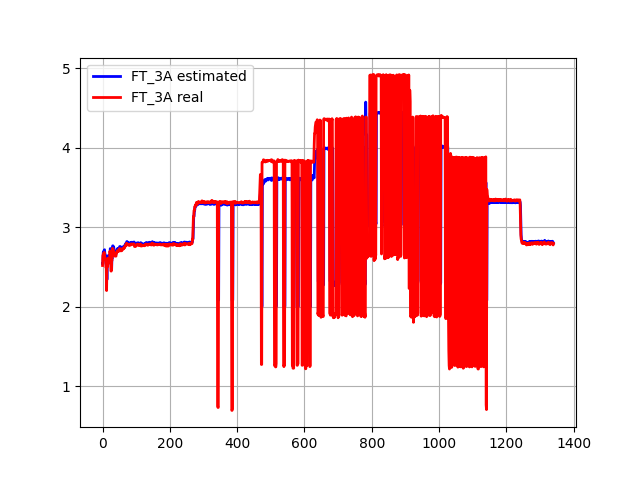
\includegraphics{results/initial-training-3A.png}
    \caption{Previsão da vazão 3A usando os dados de treinamento}
    \label{fig:initial-training-3A}
\end{figure}

Nas figuras \ref{fig:initial-training-1A} e \ref{fig:initial-training-3A} é possível ver os dados de entrada e a previsão feita pela \acrshort{rna} treinada. É gritante o nível de falhas de leituras e é devido a isto que o desempenho da RNA não foi o ideal.

Para corrigir este problema apenas duas alternativas são possíveis: analisar a planta e descobrir o que está gerando estas falhas ou implementar um filtro na entrada da \acrshort{rna}, porém ambas tarefas fogem do escopo desta disciplina.

\section{Criação do segundo modelo}
\label{sec:modelo2}

\lstinputlisting[label=code:modelo2, caption={Geração do modelo 2}]{complete.py}

O código para geração do segundo modelo é similar àquele usado para geração do primeiro, as principais diferenças não óbvias são que aqui não foi usado um único arquivo, mas sim a união dos arquivos 30hz, 35hz, 40hz, 45hz e 50hz, e que a quantidade de neurônios na camada oculta foi de 4 neurônios.

Diferente do que ocorreu no primeiro modelo, aqui os resultados encontrados foram mais interessantes: \acrshort{mse} igual a 1,35 e \acrshort{mape} de 2,2\%. Em relação ao aumento de neurônios, camadas e épocas o efeito aqui foi similar àquele encontrado antes e os resultados não melhoraram mediante estas mudanças.

\begin{figure}
    \centering
    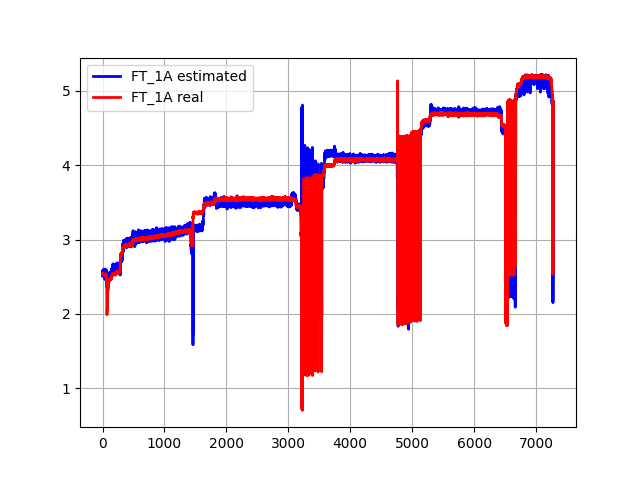
\includegraphics{results/complete-training-1A.png}
    \caption{Previsão da vazão 1A usando os dados de treinamento}
    \label{fig:complete-training-1A}
\end{figure}

\begin{figure}
    \centering
    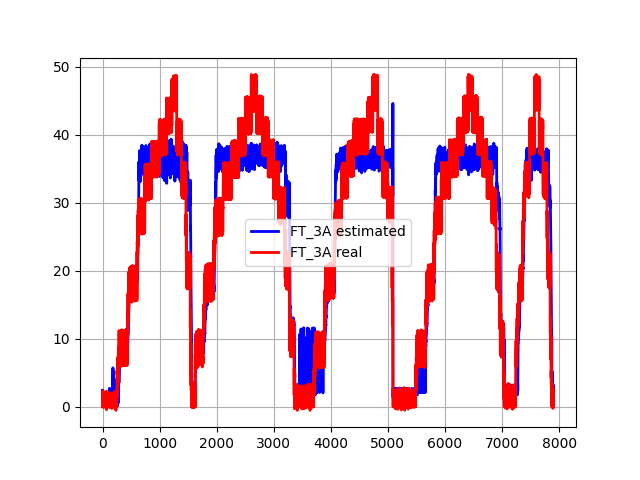
\includegraphics{results/complete-training-3A.png}
    \caption{Previsão da vazão 3A usando os dados de treinamento}
    \label{fig:complete-training-3A}
\end{figure}

Igual foi feito no modelo 1, aqui também foram geradas figuras com as previsões da \acrshort{rna} usando como entrada os dados de treinamento, são elas: \ref{fig:complete-training-1A} e \ref{fig:complete-training-3A}.
Novamente aqui o nível de medições erradas é bem alto, porém um pouco menor do que ocorreu nas medições do primeiro modelo.

\section{Teste do primeiro modelo}

\lstinputlisting[label=code:tmodelo1, caption={Teste final do primeiro modelo}]{initial-test.py}

\begin{figure}
    \centering
    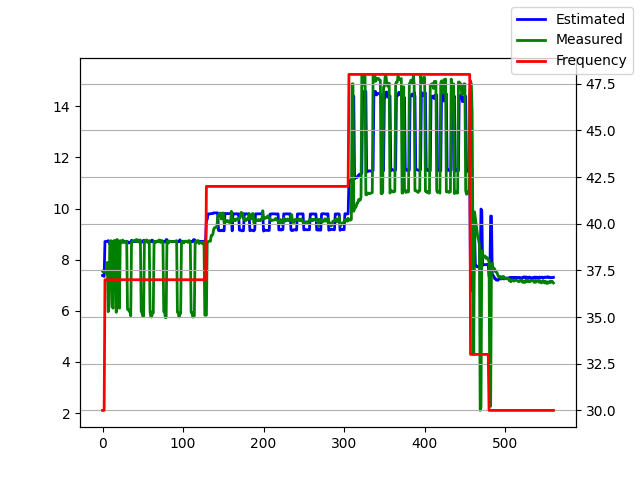
\includegraphics{results/initial-test-1A.png}
    \caption{Previsão da vazão 1A usando dados de teste, à esquerda, a escala das vazões estimada e medida, enquanto que à direita, a escala da frequência em Hertz.}
    \label{fig:initial-test-1A}
\end{figure}

\begin{figure}
    \centering
    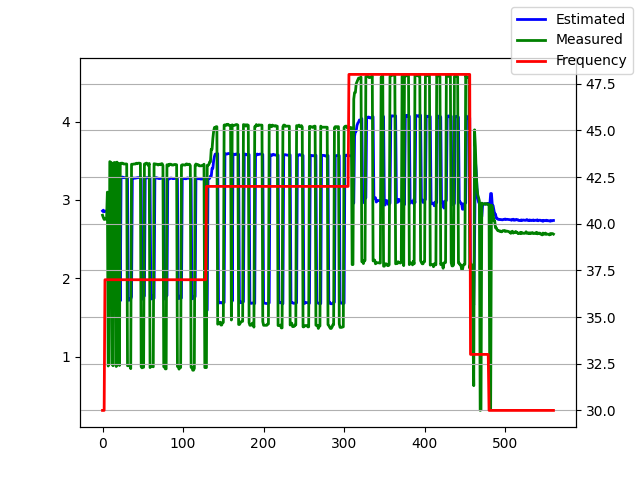
\includegraphics{results/initial-test-3A.png}
    \caption{Previsão da vazão 3A usando dados de teste, à esquerda, a escala das vazões estimada e medida, enquanto que à direita, a escala da frequência em Hertz.}
    \label{fig:initial-test-3A}
\end{figure}

Usando o código \ref{code:tmodelo1} foi possível fazer um teste da rede gerada na seção \ref{sec:modelo1}, cujo resultado pode ser visto nas figuras \ref{fig:initial-test-1A} e \ref{fig:initial-test-3A}. O \acrshort{mse} calculado foi igual a 1,35 enquanto o \acrshort{mape} foi de 22,5\%, um resultado insatisfatório devido às razões explicadas no final da seção \ref{sec:modelo1}.

\section{Teste do segundo modelo}

\lstinputlisting[label=code:tmodelo2, caption={Teste final do segundo modelo}]{complete-test.py}

\begin{figure}
    \centering
    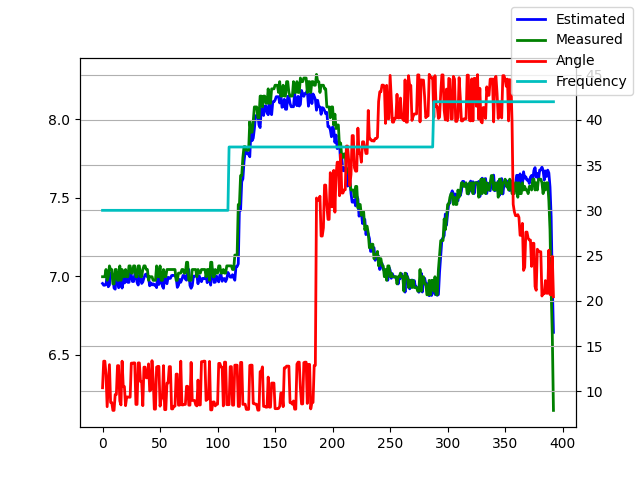
\includegraphics{results/complete-test-1A.png}
    \caption{Previsão da vazão 1A usando dados de teste, à esquerda, a escala das vazões estimada e medida, enquanto que à direita, a escala da frequência em Hertz e do ângulo da válvula em graus.}
    \label{fig:complete-test-1A}
\end{figure}

\begin{figure}
    \centering
    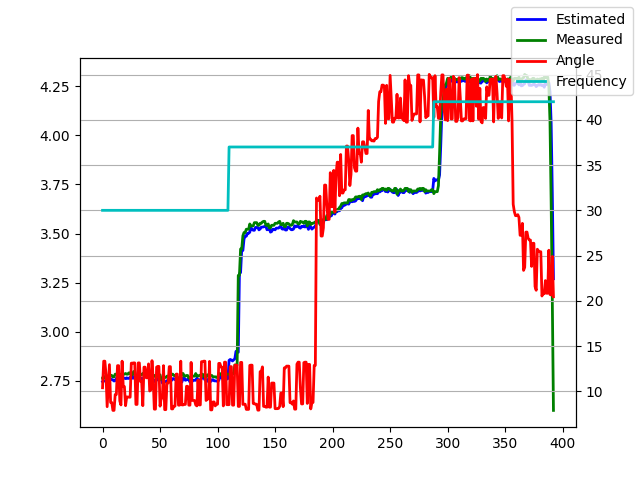
\includegraphics{results/complete-test-3A.png}
    \caption{Previsão da vazão 3A usando dados de teste, à esquerda, a escala das vazões estimada e medida, enquanto que à direita, a escala da frequência em Hertz e do ângulo da válvula em graus.}
    \label{fig:complete-test-3A}
\end{figure}

Com o código \ref{code:tmodelo2} foi feito o teste final do modelo completo, que chegou a um resultado quase perfeito, de \acrshort{mse} igual a 0,005 e \acrshort{mape} de 0,8\%. Este resultado impressionante pode ser visto nas figuras \ref{fig:complete-test-1A} e \ref{fig:complete-test-3A}.
A razão deste resultado pode ser facilmente percebida com uma rápida análise dos gráficos: este é o primeiro conjunto de dados sem erros de medição e por isso a rede neural pôde fazer as previsões com boa aproximação, mesmo tendo sido treinada com dados tão caóticos.

\section{Conclusão}

Neste trabalho foi possível ganhar experiência com o treinamento de redes neurais, processamento de dados e exibição de resultados.

A cada erro cometido uma lição foi aprendida e assim esse processo se repetiu até a conclusão da atividade.
Um exemplo de lição importante aprendida é que ao invés de começar os testes usando um grande números camadas, neurônios e épocas, o ideal é começar com a quantidade mínima e ir aumentando cada parâmetro de forma gradativa enquanto se verifica os resultados atingidos, evitando assim o superdimensionamento da rede, que muitas vezes leva a resultados piores do que redes subdimensionadas.

Por fim, sem dúvidas esta é uma ferramenta poderosa e ainda há muito mais que pode ser feito usando as \acrlong{rna}. Tudo que foi feito até agora é apenas a "ponta do iceberg" das capacidades dessa tecnologia e ainda há um longo caminho a ser percorrido até ser atingida a singularidade tecnológica.

\printglossary[type=\acronymtype]
\printglossary

\end{document}
